\documentclass[a4paper, 12pt]{article}
\usepackage{comment} % enables the use of multi-line comments (\ifx \fi) 
\usepackage{lipsum} %This package just generates Lorem Ipsum filler text. 
\usepackage{fullpage} % changes the margin
\usepackage{graphicx}
\usepackage{epsfig}
\usepackage{listings}
\usepackage{xcolor}
\lstset { %
	language=C++,
	backgroundcolor=\color{black!5}, % set backgroundcolor
	basicstyle=\footnotesize,% basic font setting
}

\begin{document}
%Header-Make sure you update this information!!!!
\noindent
\large\textbf{Lab 5 Report} \hfill \textbf{Abhishek Srivastava} \\
\normalsize CS260-001: Computer Security \hfill Student Id: 861307778 \\
\normalsize Prof. Heng Yin \hfill \today \\
\hrule

\section*{Symbolic Execution Using Angr}

\textbf{Problem 1}

The first binary \textbf{re}, when given a correct input, it will print out “right”. Please write an Angr script to find this correct input.\\

\noindent
\textbf{Solution}

\begin{lstlisting}
#!/usr/bin/env python2

# Author: Abhishek Kumar Srivastava
# Assignment 5 - Problem 1

import angr

#Address of the block we need to traverse
FIND_ADDR  = 0x0000000000400A8D

#Addresses of the blocks we have to avoid
AVOID_ADDR = (0x0000000000400A2F, 0x0000000000400A77)

def re_flag():
    #load the binary into angr project and disable auto loading libraries
    proj = angr.Project('re', load_options={"auto_load_libs": False})
    
    #entry_state constructor generates a SimState that is a generic
    #representation of the possible program states at the program 
    #entry point.
    state = proj.factory.entry_state()
    
    #To perform symbolic execution we need a Path.
    #Paths wrap states and act as interface for stepping 
    #forward and tracking their history.
    path = proj.factory.path(state)
    
    #Path group are used for symoblic execution process as it is a
    #collection of paths with various tags
    path_group = proj.factory.path_group()
    
    #find attribute tells which path to be included and avoid parameter 
    #describes which paths are to be avoided while execution
    path_group.explore(find=FIND_ADDR, avoid=AVOID_ADDR)
    
    #This is used to print the information.
    #found state is in pathgroup whose information is being dumped as output 
    return path_group.found[0].state.posix.dumps(0)

if __name__ == '__main__':
    print(re_flag())

\end{lstlisting}
Above program is used for capturing the flag. Figure 1,2 and 3 shows the screenshot of the disassembled data of the interested section of the programs. In the program you can see that we are trying to find data in a certain path and avoid other paths. I am trying the path where flag captured success indication is given. \textbf{loc\_400A87} seems to be good position to check but when checked there only half of the flag is captured may be because of the compare and jump to other location so I used the next address to check \textbf{loc\_400A8D}. I am avoiding the sections which give the wrong flag captured indications (\textbf{loc\_400A2F, loc\_400A77}).

\begin{figure}[h]
	\centering
	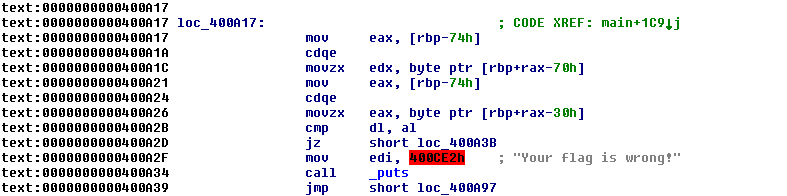
\epsfig{file=Lab_5_SS5.png, height=1.8in, width=6in}
	\caption{Output Screen Shot of disassembled path for wrong flag indication.}
\end{figure}
\begin{figure}[h]
	\centering
	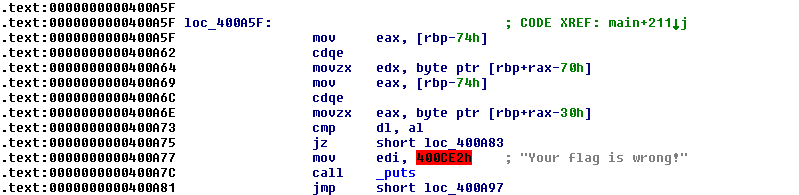
\epsfig{file=Lab_5_SS6.png, height=1.8in, width=6in}
	\caption{Output Screen Shot of disassembled path for worng flag indication.}
\end{figure}
\begin{figure}[h]
	\centering
	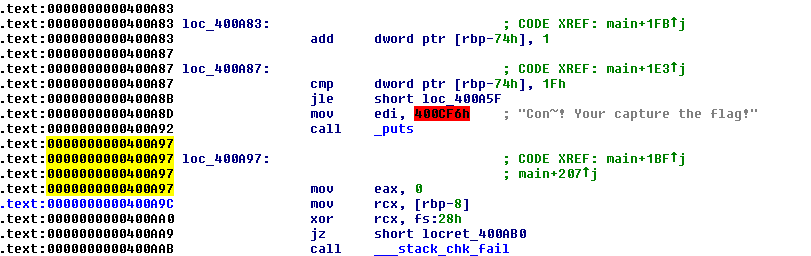
\epsfig{file=Lab_5_SS7.png, height=2in, width=6in}
	\caption{Output Screen Shot of disassembled path for correct flag captured indication.}
\end{figure}

\newpage

\begin{figure}[h]
	\centering
	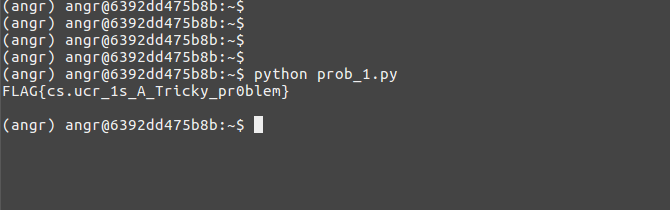
\epsfig{file=Lab_5_SS1.png, height=2in, width=6in}
	\caption{Output Screen Shot of flag captured for re.}
\end{figure}

\begin{figure}[h]
	\centering
	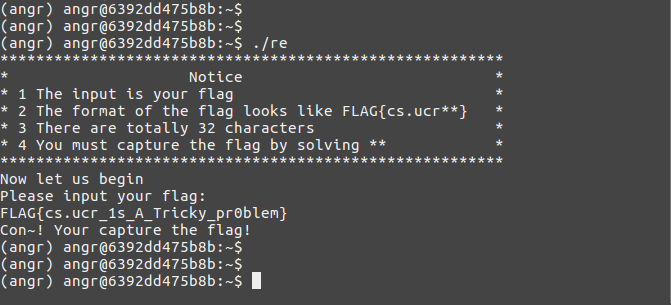
\epsfig{file=Lab_5_SS3.png, height=3in, width=6in}
	\caption{Output Screen Shot of execution when flag is entered.}
\end{figure}

Figure 4 shows the execution of the program written above on the binary provided. From this execution we captured the flag which was \textbf{FLAG\{cs.ucr\_1s\_A\_Tricky\_pr0blem\}}. To check the correctness of the flag captured I ran the program and gave the input for which I got the flag captured output from the program. Figure 5 shows the output of the execution of testing flag captured.\\

\newpage
\noindent
\textbf{Problem 2}

The second binary \textbf{afl\_strcmp} has a vulnerability. When given a right input, it will crash. Please write an Angr script to trigger the crash.\\

\noindent
\textbf{Solution}

\begin{lstlisting}
#!/usr/bin/env python2

# Author: Abhishek Kumar Srivastava
# Assignment 5 - Problem 2

import angr
#Address of the block we need to traverse
FIND_ADDR  = 0x00000000004007F9
#Addresses of the blocks we have to avoid
AVOID_ADDR = 0x000000000040080F

def main():
    #load the binary into angr project and disable auto loading libraries
    proj = angr.Project('afl_strcmp', 
                        load_options={"auto_load_libs": False})
    
    #entry_state constructor generates a SimState that is a generic
    #representation of the possible program states at the program 
    #entry point.
    state = proj.factory.entry_state()
    
    #To perform symbolic execution we need a Path.
    #Paths wrap states and act as interface for stepping 
    #forward and tracking their history.
    path = proj.factory.path(state)
    
    
    
    #Path group are used for symoblic execution process as it is a
    #collection of paths with various tags
    path_group = proj.factory.path_group()
    
    #find attribute tells which path to be included and avoid parameter 
    #describes which paths are to be avoided while execution
    path_group.explore(find=FIND_ADDR, avoid=AVOID_ADDR)
    
    #This is used to print the information.
    #found state is in pathgroup whose information is being dumped as output 
    return path_group.found[0].state.posix.dumps(0)

if __name__ == '__main__':
    print(main())

\end{lstlisting}

Above program follow the same path as the previous problem we have to identify the correct path in the program to execute angr correctly.
\begin{figure}[h]
	\centering
	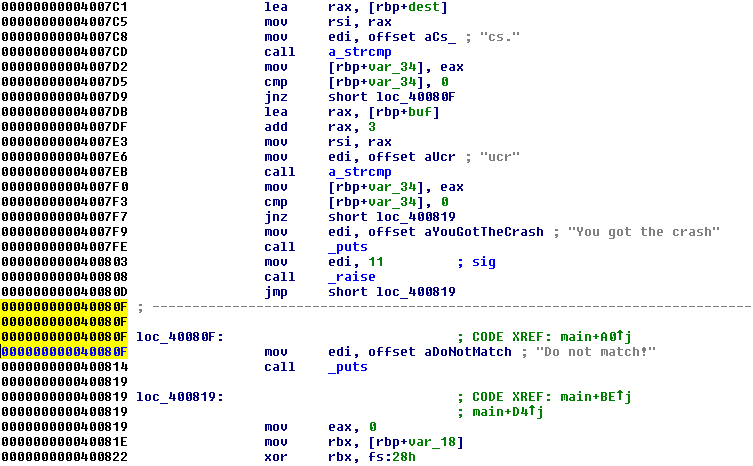
\epsfig{file=Lab_5_SS8.png, height=4in, width=6in}
	\caption{Disassembled output from IDA of the binary afl\_strcmp.}
\end{figure}

Figure 6 shows the disassembled output of the binary provided \textbf{afl\_strcmp}. Ideally we should check the path after the both string compare has been done which is \textbf{loc\_4007F0} but there are compare and jump methods are called so I tested \textbf{loc\_4007F9}. As usual I avoided the path which gives the indication of input does not match which is \textbf{loc\_40080F}.\\

Figure 7 shows the execution of the program written above. On execution we get the string whose input in the program can cause segmentation fault. To test the output captured is correct or not I ran the program and inputed the string which caused the program to give the segmentation fault indication. Figure 8 shows the execution done.
\begin{figure}[h]
	\centering
	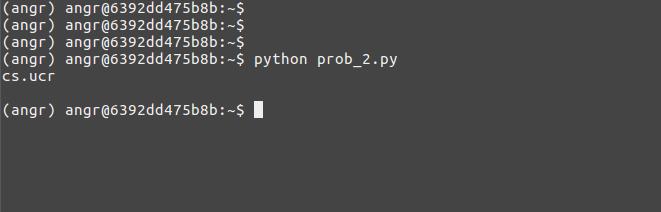
\epsfig{file=Lab_5_SS2.png, height=2in, width=6in}
	\caption{Output Screen Shot of input for program afl\_strcmp.}
\end{figure}

\begin{figure}[h]
	\centering
	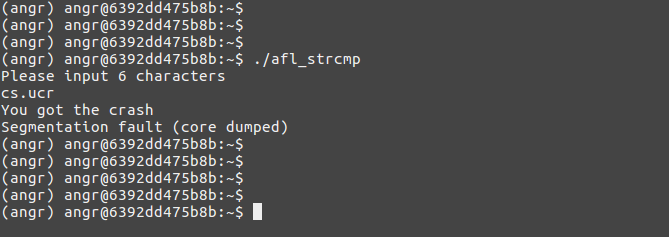
\epsfig{file=Lab_5_SS4.png, height=2.5in, width=6in}
	\caption{Output Screen Shot execution of crashing program with input captured.}
\end{figure}


\end{document}
